\documentclass[12pt]{article}
\usepackage{amsmath}
\usepackage{times}
\usepackage{graphicx}
\graphicspath{{../}}
\usepackage{color}
\usepackage{multirow}
\usepackage{placeins}
\usepackage{mathptmx} % Times-like text + math
\usepackage[T1]{fontenc}
\usepackage{hyperref}
\usepackage{makecell}
\usepackage{booktabs}
\usepackage{tabularx}
\usepackage{amsmath, amssymb}
\usepackage{array}

%%%
\usepackage{tabularx,booktabs}
\usepackage{ragged2e}
\newcolumntype{Y}{>{\RaggedRight\arraybackslash}X}

\usepackage{natbib}
\bibliographystyle{apalike}


\usepackage{setspace}
\setstretch{1.05}

\usepackage{microtype}
\setlength{\emergencystretch}{2em}

\usepackage{graphicx}
%\usepackage[authoryear]{natbib}
%
\usepackage{bbm}
\usepackage{latexsym}
%\DeclareGraphicsExtensions{.eps,.png}

%%% margins 
\textheight 23.4cm
\textwidth 14.65cm
\oddsidemargin 0.375in
\evensidemargin 0.375in
\topmargin  -0.55in
%
\renewcommand{\baselinestretch}{1.05}
%
\interfootnotelinepenalty=10000
%
\renewcommand{\thesubsubsection}{\arabic{section}.\arabic{subsubsection}}
\newcommand{\myparagraph}[1]{\ \\{\em #1}.\ \ }
\newcommand{\citealtt}[1]{\citeauthor{#1},\citeyear{#1}}
\newcommand{\myycite}[1]{\citep{#1}}

% Different font in captions
\newcommand{\captionfonts}{\normalsize}

\makeatletter  
\long\def\@makecaption#1#2{%
  \vskip\abovecaptionskip
  \sbox\@tempboxa{{\captionfonts #1: #2}}%
  \ifdim \wd\@tempboxa >\hsize
    {\captionfonts #1: #2\par}
  \else
    \hbox to\hsize{\hfil\box\@tempboxa\hfil}%
  \fi
  \vskip\belowcaptionskip}
\makeatother   
%%%%%

\renewcommand{\thefootnote}{\normalsize \arabic{footnote}} 	

\begin{document}
\hspace{13.9cm}1

\ \vspace{20mm}\\

\begin{center}{\LARGE Behavioral Latency as Weak Event-Time Supervision for EEG Reaction-Time Decoding}
\end{center}

\ \\
{\bf \large Ayana Mussabayeva$^{1}$\textsuperscript{*}}\\
ayana.mussabayeva@mbzuai.ac.ae

\ \\ {\bf \large Anuar Aimoldin$^{1}$\textsuperscript{*}}\\
anuar.aimoldin@mbzuai.ac.ae

% \ \\
% {\bf \large Ayana Mussabayeva$^{\displaystyle 1}$}\\
% ayana.mussabayeva@mbzuai.ac.ae


% \ \\ {\bf \large Anuar Aimoldin$^{\displaystyle 1}$}\\
% anuar.aimoldin@mbzuai.ac.ae

\ \\ {\bf \large Yedige Mussabayev$^{\displaystyle 2}$}\\
ymussabayev@hof-university.de

\ \\ {\bf \large Xue Liu$^{\displaystyle 1, 3}$}\\
steve.liu@mbzuai.ac.ae

\ \\ {\bf \large Kun Zhang$^{\displaystyle 1, 4}$}\\
kun.zhang@mbzuai.ac.ae


\ \\
{$^{\displaystyle 1}$Mohamed bin Zayed University of Artificial Intelligence (MBZUAI), Abu Dhabi, UAE}
\ \\
{$^{\displaystyle 2}$ Hof University, Hof, Germany}
\ \\
{$^{\displaystyle 3}$ McGill University, Montreal, QC, Canada}
\ \\
{$^{\displaystyle 4}$ Carnegie Mellon University, Pittsburgh, PA, USA}
\ \\
{\normalsize \textsuperscript{*}Equal contribution}\\




\ \\[-2mm]
{\bf Keywords:} weak event-time supervision, event-time posterior modeling, EEG reaction-time decoding, behavioral latency, shifted-crop diagnostics

\thispagestyle{empty}
\markboth{}{NC instructions}
%
\ \vspace{-0mm}\\
%
%Abstract
\begin{center} {\bf Abstract} \end{center}



Single-trial EEG analyses are often organized around events and latencies, such as stimulus onset, response execution, ERP component timing, and movement onset. Yet EEG-based reaction-time prediction is commonly formulated as scalar regression from a fixed stimulus-locked window, treating reaction time as a label attached to the whole segment rather than as behavioral evidence about when response-relevant dynamics are expressed within post-stimulus EEG. Here we reformulate trial-wise reaction-time decoding as event-time posterior modeling. Instead of predicting a single RT directly, the model estimates a posterior distribution over response-relevant event times, \(p(t_{\mathrm{event}} \mid X)\), and reads out RT as the posterior expectation. This treats behavioral latency as a weak observation of latent response-relevant timing and makes the output representation, not only the architecture, part of the computational hypothesis.

We test this output-space hypothesis on the Healthy Brain Network contrast change detection EEG task under a subject-disjoint, release-separated protocol. Architecture and readout controls show that the gain is not explained by architecture scale or by a differentiable expectation readout alone. Distributional event-time supervision yields lower held-out error than the strongest scalar and temporal-readout baselines. Loss ablations and five-seed checks support the interpretation that the gain comes from supervising the event-time distribution, not merely from using a soft-argmax readout. EventNLL provides a probabilistic latent-event alternative, treating observed RT as a noisy realization of an unobserved response-relevant event time.

Beyond point prediction, the event-time posterior becomes a diagnostic object for separating temporal evidence from scalar shortcuts. Posterior width, target-aligned mass, mode-mean disagreement, and interval coverage characterize whether predictions are localized, diffuse, overconfident, or miscalibrated. We further introduce shifted-crop inference as a shortcut-vs-localization diagnostic. A matched shift-jitter intervention improves shifted-crop robustness and localizer-like movement, but sensitivity remains far from ideal crop-relative localization. Together, these results support event-time posterior modeling as a probabilistic and interpretable formulation for linking single-trial EEG dynamics to behavioral timing. The same event-time view is naturally relevant to EEG settings in which the target has a latency interpretation, including ERP latency estimation, movement onset decoding, and other latency-varying neural or behavioral phenomena.






\section{Introduction}

Behavioral timing provides a direct link between neural dynamics and behavior. In reaction-time (RT) tasks, the observed response latency reflects sensory encoding, decision formation, motor preparation, and response execution unfolding over hundreds of milliseconds. EEG analyses often exploit this temporal structure through event alignment, response locking, and latency variability; trial-to-trial latency variation can carry behaviorally meaningful information that is obscured by averaging or by models that collapse temporal structure into window-level labels \citep{Jung1998SingleTrialERP,Ouyang2017LatencyReview}.

Supervised EEG decoding, however, often treats a fixed stimulus-locked window as an input to a class label or scalar behavioral variable. For RT decoding, this means that a delayed behavioral response latency is treated as a property of the whole EEG segment. A scalar predictor may therefore achieve low error by learning subject-level slowness, trial difficulty, or stimulus-locked response tendencies without representing when response-relevant dynamics are expressed within the window.

We address this mismatch by treating behavioral RT as weak event-time supervision. The button press is not a direct annotation of neural event onset; it is a noisy behavioral observation produced by sensory, decision, and motor processes. Nevertheless, it constrains the timing of response-relevant dynamics. Given an EEG window \(X\), the model estimates a posterior distribution \(p(t_{\mathrm{event}}\mid X)\) over response-relevant event times and derives the scalar RT prediction as the posterior expectation. This keeps compatibility with standard scalar metrics such as nRMSE while making the timing semantics of RT explicit.

This formulation is complementary to work on stronger EEG architectures, self-supervised pretraining, and foundation-style EEG models, which target representation learning across subjects, tasks, and recording setups \citep{wang2024eegpt,Jiang2024LaBraM,Chen2024EEGFormer,Wang2025EEGMamba,ElOuahidi2025REVE,Yue2024BrainGPT}. We ask a different question: when the target is a behavioral latency, can changing the output space from a scalar to a latent event-time posterior change both what the model learns and what evidence can be inspected?

We study this question on the Healthy Brain Network contrast change detection EEG task \citep{Shirazi2024HBNEEG}, following the RT prediction setting introduced by the EEG Foundation Challenge \citep{EEGFoundationChallengeArxiv2025,EEGChallengeWebsite2025}. Under a subject-disjoint, release-separated protocol, we compare direct scalar regression, temporal-readout regression, soft-argmax RT-loss controls, and distributionally supervised event-time models. This control structure separates architecture capacity, differentiable expectation readout, scalar timing loss with a temporal head, and full posterior supervision.

The posterior view also changes what can be evaluated from each trial. Posterior width, target-aligned mass, mode-mean disagreement, and interval coverage characterize localization, uncertainty, and calibration even when scalar errors are similar. We further introduce shifted-crop inference as a shortcut-vs-localization diagnostic: a crop-relative timing localizer should shift its predicted crop-relative response time opposite to the crop shift, whereas a crop-invariant scalar shortcut should remain closer to fixed absolute timing.

Our results support this event-time formulation. Distributional event-time supervision improves held-out prediction over scalar and temporal-readout controls, remains stable in five-seed checks, and is not explained by soft-argmax alone. Posterior-geometry and shifted-crop analyses reveal temporal evidence and partial response-timing localization behavior hidden by scalar metrics, while shift-jitter training reduces fixed-window shortcut behavior without solving full crop-relative timing localization. Although our experiments focus on RT prediction, the same event-time view is relevant to EEG targets with latency semantics, including ERP latency estimation, movement onset decoding, error-related responses, and other latency-varying phenomena.

Our contributions are:
\begin{enumerate}
    \item We recast behavioral RT as weak event-time supervision and formulate EEG RT decoding as event-time posterior modeling rather than direct scalar regression.
    \item We evaluate this formulation under a subject-disjoint, release-separated HBN-EEG protocol designed to separate EEG backbone capacity, temporal readout parameterization, and distributional event-time supervision.
    \item We show through controlled baselines and loss ablations, with seed-level variability reported for the main comparisons, that distributional event-time supervision improves over scalar regression, temporal-readout regression, and soft-argmax RT-loss controls. We also evaluate EventNLL as a latent event-time likelihood in which observed RT is treated as a noisy realization of an unobserved response-relevant event.
    \item We turn the learned event-time posterior into a temporally resolved evaluation object: posterior geometry separates scalar accuracy from temporal concentration and interval behavior, while shifted-crop diagnostics and shift-jitter training test shortcut behavior and partial response-timing localization.
\end{enumerate}

\section{Related Work}

\subsection{Event-Centered EEG Analysis and Latency Variability}
EEG is often analyzed through events and latencies. Stimulus onset, response execution, error-related activity, movement onset, ERP component timing, and other temporally localized phenomena define not only what occurs in a trial, but also when task-relevant neural or behavioral processes unfold. This event-centered view appears in annotation systems such as Hierarchical Event Descriptors \citep{BigdelyShamlo2016HED} and in single-trial ERP analysis, where ERP-image visualization and related methods show that sorting trials by RT can reveal performance-linked temporal structure \citep{Jung1998SingleTrialERP}. RIDE and subsequent reviews further emphasize that intra-subject ERP latency variability can be estimated and can carry behavioral meaning \citep{Ouyang2011RIDE,Ouyang2017LatencyReview}.

Response- and movement-related EEG provide related examples. Lateralized readiness potentials index response preparation and execution \citep{Coles1989LRP}; error-related negativities provide response-locked signatures of error commission and performance monitoring \citep{Gehring1993ErrorDetection,HolroydColes2002ERN}; and movement-related cortical potentials, including the Bereitschaftspotential, organize EEG dynamics around movement onset and premovement preparation \citep{KornhuberDeecke1965BP,ShibasakiHallett2006BP}. Decision-time models make a related point at the behavioral level by treating RT variability as a consequence of latent temporal dynamics in evidence accumulation and decision formation \citep{Ratcliff2008Diffusion,OConnell2012Supramodal,Kelly2013Internal}. We do not fit such a cognitive process model; we use the weaker premise that observed RT is a noisy behavioral latency associated with an unobserved response-relevant event time.

Explicit EEG event detection is also well established when annotated onsets, offsets, or intervals are available. Sleep-event detectors, for example, estimate when transient events such as spindles and K-complexes occur rather than predicting only a window-level label \citep{Chambon2019DOSED,TapiaRivas2024SEED}. Our setting differs because we do not begin with manually annotated neural event times; RT is recorded as a scalar but provides weak time-of-occurrence evidence.

\subsection{Fixed-Window EEG Decoding of Latency-Structured Targets}
Modern supervised EEG decoding often maps a fixed stimulus-locked or task-locked EEG window to a scalar or class label. This formulation is convenient and aligns with benchmark metrics, but it can collapse temporal structure when the target itself has time-of-occurrence semantics. RT is evaluated as one scalar per trial, yet it denotes the latency of a behavioral response following stimulus onset.

EEG-based RT estimation has commonly followed this scalar-prediction form, including regression pipelines based on Riemannian geometry features \citep{Wu2017RiemannianRT} and deep single-trial EEG models for visual-stimulus RT prediction \citep{Chowdhury2020RTSensors}. The EEG Foundation Challenge provides a standardized scalar benchmark using normalized RMSE \citep{EEGFoundationChallengeArxiv2025,EEGChallengeWebsite2025}. We keep this scalar evaluation protocol, but ask whether the same label can be used internally as weak event-time supervision. This distinction matters because a scalar regressor may learn trial difficulty, subject-level response tendency, or stimulus-locked temporal priors without representing where response-relevant dynamics are expressed. A temporal soft-argmax readout alone also does not resolve the issue if the model is still trained only through scalar RT error.

\subsection{Distributional and Time-to-Event Output Modeling}
Latency-structured EEG targets also motivate output distributions rather than only point estimates. Label distribution learning replaces a hard label with a distribution over related labels, which is useful when neighboring labels share metric structure or when ambiguity is meaningful \citep{Geng2016LabelDistributionLearning}. For RT, neighboring labels are ordered time bins, making a smoothed event-time distribution a natural supervision target.

Time-to-event modeling provides a complementary probabilistic language for ordered event times. Classical survival analysis and neural time-to-event models estimate distributions over event times rather than only scalar predictions or risk scores \citep{Cox1972CoxPH,Lee2018DeepHit}. Distributional evaluation also makes uncertainty and calibration observable through posterior width, coverage, likelihood scores, and proper scoring rules \citep{Chapfuwa2023Calibration,Haider2020SurvivalDistributions}. We use this literature locally for finite EEG windows, not as a standard survival-analysis setting with long-horizon risk, censoring, or competing clinical outcomes. EventNLL instantiates this view by treating observed RT as a noisy realization of a latent response-relevant event time.

\subsection{Relation to EEG Backbones, Pretraining, and Robust Decoding}
A separate line of EEG decoding work addresses cross-subject, cross-session, and cross-dataset variability through stronger input representations. Classical approaches include Riemannian covariance-based decoding and alignment methods for reducing subject or session mismatch \citep{Barachant2012RiemannianBCI,Jayaram2016TransferLearningBCI,Zanini2018RiemannianTL,HeWu2020EuclideanAlignment}. Deep learning approaches pursue related goals through domain adaptation, moment matching, supervised EEG architectures, self-supervised pretraining, and foundation-style EEG backbones \citep{Ganin2016DANN,SunSaenko2016DeepCORAL,Kostas2021BENDR,wang2024eegpt,Jiang2024LaBraM,Chen2024EEGFormer,Wang2025EEGMamba,ElOuahidi2025REVE,Yue2024BrainGPT}.

Our contribution is complementary to these input-representation approaches. We do not propose a new general-purpose EEG backbone, invariant representation loss, or pretraining strategy. Instead, we focus on output representation and supervision: when the target is a latency, the label is not only a scalar value to regress, but also weak evidence about when response-relevant dynamics are expressed. External EEG architectures and foundation-style models trained from scratch therefore serve as controlled architecture baselines. What remains missing in prior work is a controlled EEG RT formulation that connects scalar benchmark evaluation, temporal-readout controls, distributional event-time supervision, and posterior-level diagnostics. We fill this gap by learning a posterior over response-relevant latencies and evaluating it as temporal evidence rather than only as a source of a scalar RT estimate.


\section{Dataset and Evaluation Protocol}
\label{sec:dataset_protocol}

\subsection{HBN-EEG CCD Reaction-Time Task}

We use the reaction-time prediction task introduced by the NeurIPS EEG Foundation Challenge \citep{EEGChallengeWebsite2025,EEGFoundationChallengeArxiv2025}, based on curated releases of the HBN-EEG dataset \citep{Shirazi2024HBNEEG}. Our analysis is restricted to the contrast change detection (CCD) reaction-time subset rather than the full multi-task HBN-EEG resource.

In the CCD task, participants viewed two flickering grating stimuli and responded after a contrast change made one grating perceptually dominant. The released target is the trial-wise reaction time from stimulus onset to button press. Each main experiment uses the same fixed 2~s stimulus-locked EEG window spanning 0.5--2.5~s after stimulus onset, sampled at 100~Hz from 128 EEG channels after excluding the reference channel. Thus each input has \(T=200\) samples. Because RT marks when a response occurs within this post-stimulus window, the task naturally supports an event-time interpretation rather than only a window-level scalar regression view.

\begin{figure}[!t]
    \centering
    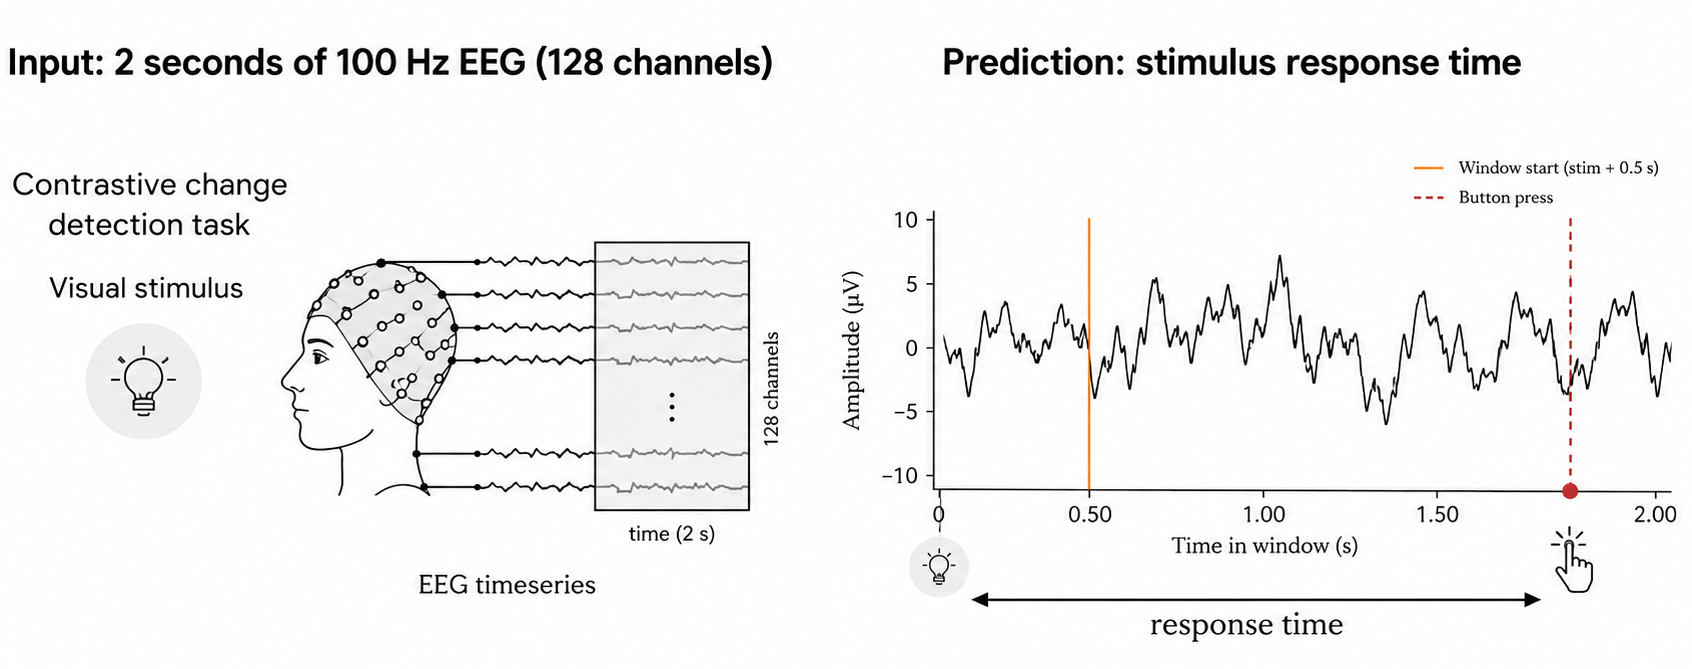
\includegraphics[width=0.9\linewidth]{img/challenge_task.png}
    \caption{HBN-EEG contrast change detection reaction-time task. Each trial provides a stimulus-locked EEG segment and a trial-wise RT target from stimulus onset to button press.}
    \label{fig:tasks}
\end{figure}


\subsection{Shared Evaluation Protocol}

We use this task as a controlled evaluation setting for separating three possible sources of RT prediction performance: EEG backbone capacity, temporal readout parameterization, and distributional event-time supervision. The benchmark therefore fixes the data split, target support, input representation, and scalar evaluation rule before varying architectures and objectives in the subsequent model and diagnostic sections.

To avoid subject leakage, all models use the same release-separated CCD split: R1--R8 for fitting, R9--R10 for development choices such as early stopping, checkpoint selection, readout-temperature tuning, and protocol diagnostics where applicable, and R11 as a one-shot final holdout after all model and readout choices are fixed. R11 holdout labels are not used for model fitting, checkpoint selection, readout-temperature selection, or protocol decisions. For consistency, the main analyzed set includes only trials whose response lies inside the fixed 2~s window (\(0.5 \leq \mathrm{RT} \leq 2.5\)~s). Table~\ref{tab:ccd_protocol_stats} reports the resulting partitions; metadata checks confirmed zero subject overlap across train, development, and holdout after filtering.

\begin{table}[!t]
\centering
\caption{Release-separated CCD protocol statistics after window construction and RT-support filtering. Prepared trials are 2~s CCD windows with stimulus and response annotations; analyzed trials additionally satisfy \(0.5 \leq \mathrm{RT} \leq 2.5\)~s.}
\label{tab:ccd_protocol_stats}
\setlength{\tabcolsep}{3pt}
\renewcommand{\arraystretch}{1.12}
\begin{tabular*}{\linewidth}{@{\extracolsep{\fill}} l l r r r @{}}
\toprule
\textbf{Partition} & \textbf{Releases} & \textbf{Prepared trials} & \textbf{Analyzed trials} & \textbf{Subjects} \\
\midrule
Train & R1--R8 & 74{,}576 & 73{,}030 & 1{,}221 \\
Development & R9--R10 & 17{,}867 & 17{,}348 & 308 \\
Holdout & R11 & 15{,}751 & 15{,}164 & 292 \\
\bottomrule
\end{tabular*}
\end{table}

The main analysis keeps trials whose behavioral RT falls inside the modeled event-time support, 0.5--2.5~s after stimulus onset. This filter removes 1{,}546/74{,}576 training trials (2.07\%), 519/17{,}867 development trials (2.90\%), and 587/15{,}751 holdout trials (3.73\%). In the prepared CCD split artifacts, excluded trials are fast responses below 0.5~s; no prepared trial has RT above 2.5~s. The conclusions therefore apply to support-representable responses in the analyzed post-stimulus window, and should not be interpreted as claims about very fast anticipatory responses or RT regimes outside the represented support.

Scalar performance is evaluated using normalized RMSE (nRMSE), defined as RMSE divided by the standard deviation of the true targets within the evaluated split \citep{EEGChallengeWebsite2025}. Main scalar comparisons use the same support-filtered R9--R10 development set and final holdout set. Diagnostic analyses that require shifted crop starts, stricter RT support, or posterior-only summaries are introduced locally in the corresponding subsection or appendix and do not affect the main holdout reporting protocol.

\begin{table}[!t]
\centering
\caption{Controlled comparison and diagnostic blocks under the shared protocol. The first two blocks define the main scalar-performance comparisons; the final block evaluates posterior readout, posterior geometry, and shortcut-vs-localization behavior after event-time models have been trained.}
\label{tab:experiment_map}
\scriptsize
\setlength{\tabcolsep}{2pt}
\renewcommand{\arraystretch}{1.08}
\begin{tabularx}{\linewidth}{@{} >{\RaggedRight\arraybackslash}p{0.15\linewidth} >{\RaggedRight\arraybackslash}p{0.18\linewidth} >{\RaggedRight\arraybackslash}p{0.18\linewidth} >{\RaggedRight\arraybackslash}p{0.14\linewidth} >{\RaggedRight\arraybackslash}X @{}}
\toprule
\textbf{Comparison block / model family} & \textbf{Model capacity} & \textbf{Temporal readout} & \textbf{Supervision} & \textbf{Role} \\
\midrule
\multicolumn{5}{@{}l}{\textit{Scalar regression controls}} \\
\addlinespace[0.15em]
External EEG backbones & Standard EEG architectures trained from scratch & Scalar RT head & Scalar RT & Assesses whether generic EEG backbone capacity explains performance. \\
MSP-CNN family & Compact scalar CNN & Segment-pooling scalar readout & Scalar RT & Scalar baseline with coarse temporal pooling. \\
ETR-CNN family & Compact scalar CNN & Temporal expectation readout & Scalar RT & Isolates temporal expectation readout under scalar RT supervision. \\
\midrule
\multicolumn{5}{@{}l}{\textit{Event-time objective comparison}} \\
\addlinespace[0.15em]
Soft-argmax RT-loss control & Shared segmentation backbone & Posterior-mean readout & Scalar RT only & Isolates posterior-mean readout without distributional supervision. \\
CE soft-target objective & Shared segmentation backbone & Posterior-mean readout & Soft event-time target & Direct soft-label event-time supervision. \\
Likelihood-based objectives & Shared segmentation backbone & Posterior-mean readout & Latent event-time likelihood & Probabilistic latent-event supervision. \\
Wasserstein control & Shared segmentation backbone & Posterior-mean readout & Distributional geometry loss & Alternative geometry-based distributional supervision. \\
\midrule
\multicolumn{5}{@{}l}{\textit{Posterior and localization diagnostics}} \\
\addlinespace[0.15em]
Readout-temperature tuning & Trained event-time models & Temperature-adjusted posterior mean & Learned posterior & Standardizes scalar posterior-mean readout. \\
Posterior geometry diagnostics & Trained event-time models & Posterior summaries & Learned posterior & Exposes posterior structure beyond scalar nRMSE. \\
Shifted-crop diagnostic & Trained fixed-window models & Crop-relative posterior mean & No new training & Probes shortcut-vs-localization behavior. \\
Shift-jitter intervention & Matched event-time models & Crop-relative posterior mean & Shifted crop-relative targets & Intervenes on crop-start variation to improve robustness and localizer-like movement. \\
\bottomrule
\end{tabularx}
\end{table}

Table~\ref{tab:experiment_map} maps the shared protocol to the comparison blocks used below. The scalar regression controls vary compact temporal regressors and external EEG backbones under scalar RT supervision. The event-time objective comparison fixes the ETS-U-Net backbone and varies the output supervision. Posterior geometry, shifted-crop inference, and shift-jitter training are diagnostic extensions applied after training; they evaluate posterior semantics and shortcut-vs-localization behavior rather than defining a separate scalar benchmark family.

\subsection{Shared Training, Readout Tuning, and Inference Protocol}
\label{sec:shared_protocol}

To support this controlled comparison, we keep preprocessing, optimization, augmentation, checkpointing, and inference fixed wherever possible, so that the main experimental axes remain EEG backbone capacity, temporal readout parameterization, and distributional event-time supervision. All neural models receive the same input normalization: for each 2~s trial window and EEG channel, we subtract the channel's temporal mean within the window and divide by its temporal standard deviation within the same window. The shared training recipe uses Adam with learning rate \(10^{-3}\), zero weight decay, train batch size 128, up to 100 epochs, and early stopping on development nRMSE with patience 20.

Unless otherwise stated, training uses one fixed augmentation profile, so that regularization is not a model-specific tuning degree of freedom. The profile combines channel dropout, temporal cutout, and Gaussian noise with the same settings for all supervised neural models. Regression models use scalar RT supervision, while event-time models represent RT either as a soft crop-relative event-time target or as an observation under a latent event-time likelihood. When temperature scaling is used for event-time posterior readout, \(\tau\) is selected on R9--R10 to minimize development nRMSE of the posterior-mean readout and then applied unchanged to the holdout split. The main regression-baseline and event-time-objective comparisons are repeated over five seeds (2025--2029).

\section{Scalar Regression Controls}
\label{sec:baseline_regression}

The regression baselines establish how far scalar supervision can go before introducing event-time targets. We separate two types of controls: compact task-specific temporal controls and supervised external EEG backbones trained from scratch under the same protocol.

The compact controls form a progression of window-level temporal inductive biases. MSP-CNN (multiscale segment-statistic pooling CNN; Figure~\ref{fig:ch1_regression}) explicitly accounts for temporal structure by collecting mean and max statistics from coarse temporal segments of the feature map. These segment-level summaries act as early/middle/late activation cues and are mapped to scalar RT. ETR-CNN (event-time readout CNN) turns this coarse temporal summary into a learned time-indexed readout: it preserves temporal scores over the input window and predicts RT as the expected time under learned time-bin weights. ETR-CNN large keeps the same readout while increasing feature capacity.

We compare these task-specific regressors with external EEG architectures adapted to scalar RT regression. These include classical convolutional EEG baselines, Deep4Net and ShallowFBCSPNet \citep{braindecode}; the compact EEGNet architecture \citep{lawhern2018eegnet}; TIDNet's thinker-invariant convolutional design \citep{kostas2020thinkerinvariance}; the convolutional-transformer EEGConformer \citep{song2023eegconformer}; the attention temporal convolutional ATCNet architecture \citep{altaheri2022atcnet}; EEGPT \citep{wang2024eegpt}; Medformer \citep{wang2024medformer}; and the LaBraM foundation-style architecture \citep{Jiang2024LaBraM}. All external architectures are trained from scratch; pretrained weights are not used.

ETR-CNN large is the strongest scalar baseline, with MSP-CNN and base ETR-CNN close behind. The external EEG backbones train meaningfully but do not close the gap to these compact temporal controls, suggesting that task-specific temporal structure matters more for this RT task than generic backbone capacity alone. These results provide strong scalar controls for the next step: testing whether directly supervising an event-time distribution improves beyond scalar RT training.

\begin{figure}[!t]
    \centering
    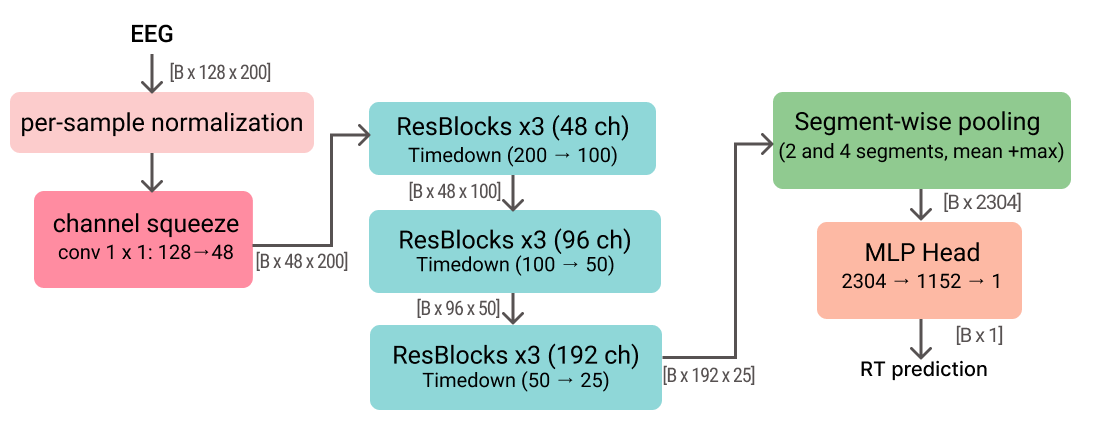
\includegraphics[width=\linewidth]{img/ch1/Ch1_regression.png}
    \caption{MSP-CNN direct RT regression baseline architecture. A lightweight 1-D temporal ConvNet maps an EEG trial window to a scalar reaction-time prediction. A learned $1\times1$ channel-squeeze layer (128$\rightarrow$48) is followed by residual depthwise-separable stages with anti-aliased temporal downsampling, segment-wise pooling (2 and 4 segments; mean+max), and an MLP head.}
    \label{fig:ch1_regression}
\end{figure}

\begin{table}[!t]
\centering
\caption{Direct-regression and wrapped external backbone baselines. Values are mean $\pm$ sample standard deviation.}
\label{tab:r11_regression_baselines}
\footnotesize
\setlength{\tabcolsep}{2pt}
\renewcommand{\arraystretch}{1.15}
\begin{tabularx}{\linewidth}{@{} >{\RaggedRight\arraybackslash}p{0.22\linewidth} Y >{\centering\arraybackslash}p{0.215\linewidth} >{\centering\arraybackslash}p{0.215\linewidth} @{}}
\toprule
\textbf{Model} & \textbf{Role} & \textbf{Valid nRMSE} $\downarrow$ & \textbf{Holdout nRMSE} $\downarrow$ \\
\midrule
\multicolumn{4}{@{}l}{\textit{Task-specific regression baselines}} \\
\addlinespace[0.15em]
MSP-CNN & segment-pooling scalar & \mbox{0.9006 $\pm$ 0.0051} & \mbox{0.8998 $\pm$ 0.0080} \\
ETR-CNN & temporal readout & \mbox{0.9008 $\pm$ 0.0060} & \mbox{0.8977 $\pm$ 0.0068} \\
ETR-CNN large & capacity ablation & \textbf{\mbox{0.8972 $\pm$ 0.0040}} & \textbf{\mbox{0.8928 $\pm$ 0.0042}} \\
\midrule
\multicolumn{4}{@{}l}{\textit{External regression baselines}} \\
\addlinespace[0.15em]
TIDNet & thinker-invariant CNN & \mbox{0.9235 $\pm$ 0.0024} & \textbf{\mbox{0.9192 $\pm$ 0.0027}} \\
EEGConformer & conv-transformer & \textbf{\mbox{0.9188 $\pm$ 0.0026}} & \mbox{0.9287 $\pm$ 0.0057} \\
EEGNet & compact CNN & \mbox{0.9350 $\pm$ 0.0054} & \mbox{0.9335 $\pm$ 0.0028} \\
LaBraM & foundation-style & \mbox{0.9304 $\pm$ 0.0061} & \mbox{0.9327 $\pm$ 0.0086} \\
Deep4Net & deep ConvNet & \mbox{0.9269 $\pm$ 0.0045} & \mbox{0.9260 $\pm$ 0.0044} \\
ShallowFBCSPNet & shallow FBCSP CNN & \mbox{0.9324 $\pm$ 0.0016} & \mbox{0.9343 $\pm$ 0.0024} \\
ATCNet & conv/attention/TCN & \mbox{0.9686 $\pm$ 0.0183} & \mbox{0.9666 $\pm$ 0.0151} \\
EEGPT & foundation-style & \mbox{0.9616 $\pm$ 0.0201} & \mbox{0.9584 $\pm$ 0.0185} \\
Medformer & larger transformer & \mbox{0.9623 $\pm$ 0.0046} & \mbox{0.9585 $\pm$ 0.0051} \\
\bottomrule
\end{tabularx}
\end{table}

\section{Event-Time Posterior Formulation}
\label{sec:event_time_formulation}

To make response timing explicit, we reformulate RT prediction as event-time posterior modeling. Instead of predicting a scalar directly, the model produces per-time logits and a posterior distribution over response-relevant event times; scalar RT is then read out as the posterior expectation. The key distinction from temporal-readout regression is that the objective directly supervises the distributional event-time representation, rather than using a temporal head only as a scalar-regression readout.

We evaluate two ways of turning scalar RT labels into event-time supervision. The first constructs an explicit soft target distribution over time, asking the model to match a smoothed target centered at the observed RT. The second treats the observed RT statistically, as a noisy observation of an unobserved response-relevant event time, and optimizes a latent event-time likelihood. These two families correspond to soft-target objectives and likelihood-based objectives, respectively.

The core event-time experiments are designed to isolate the role of output formulation. The regression controls above test how far scalar supervision can go with task-specific temporal readouts and external EEG backbones. Here, we fix the event-time segmentation U-Net (ETS-U-Net) backbone and vary the event-time objective, so that differences in scalar accuracy, posterior geometry, and diagnostic behavior under temporal crop shifts reflect how RT is supervised over time rather than which architecture is used. Figure~\ref{fig:event_time_scheme} summarizes this pipeline from fixed-window EEG input to weak event-time supervision, posterior readout, and shifted-crop diagnostics.

\begin{figure}[!t]
    \centering
    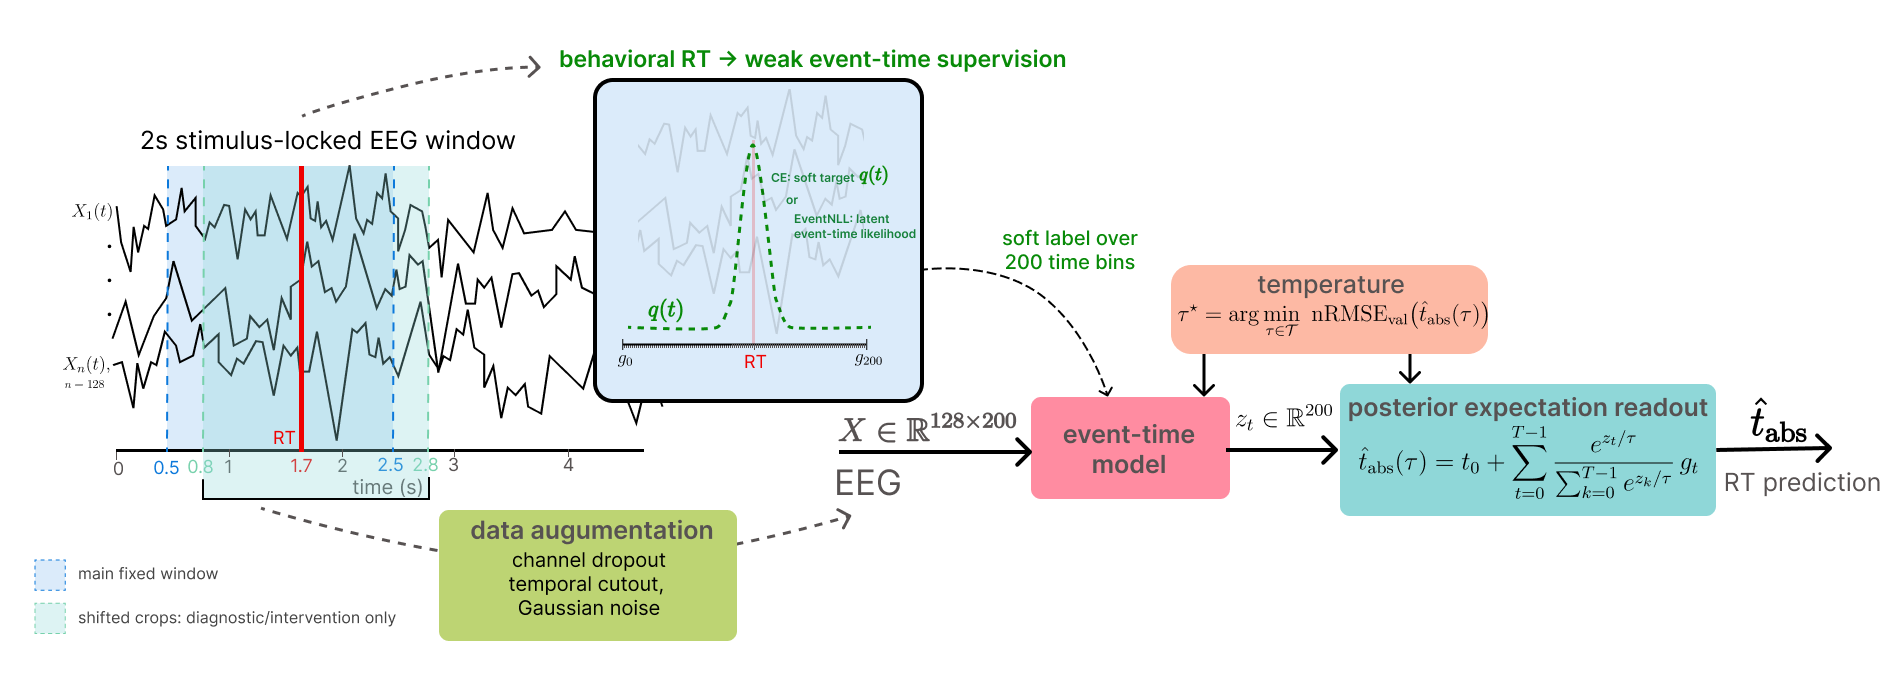
\includegraphics[width=\linewidth]{img/ch1/event_time_scheme.png}
    \caption{Event-time posterior formulation for EEG reaction-time prediction. A fixed 0.5--2.5~s stimulus-locked EEG window is mapped to time-bin logits, and behavioral RT provides weak event-time supervision either through a soft target distribution or a latent EventNLL likelihood. Scalar RT is read out as the posterior expectation after selecting a readout temperature on R9--R10. Shifted crops are used only for diagnostic and shift-jitter intervention analyses. The schematic shows the categorical posterior readout; the hazard EventNLL variant uses a hazard-derived probability mass function with the same expectation readout.}
    \label{fig:event_time_scheme}
\end{figure}

\subsection{Event-Time Segmentation Architecture}
\label{sec:event_time_architectures}

ETS-U-Net maps an EEG trial window
$X\in\mathbb{R}^{C\times T}$ to per-time logits $z_{0:T-1}$ (Figure~\ref{fig:ets_unet}). It follows a 1-D U-Net style encoder-decoder with skip
connections for precise localization \citep{ronneberger2015unet}. The encoder progressively downsamples the temporal axis
to build multi-scale context, while the decoder upsamples and fuses encoder features to recover per-time outputs at the
input temporal resolution (internal down/up-sampling is used only to form multi-scale features). Each scale is refined
with lightweight residual blocks (ResNet-style skips) \citep{he2016resnet} built from depthwise-separable 1-D convolutions
for computational efficiency \citep{howard2017mobilenets,chollet2017xception}. To mitigate aliasing under temporal
decimation, downsampling applies a fixed depthwise smoothing filter followed by strided averaging (``blur-pool'' style)
\citep{zhang2019shiftinvariant}. A dilated bottleneck further enlarges the receptive field without additional downsampling
\citep{yu2016dilated}.

\begin{figure}[t]
    \centering
    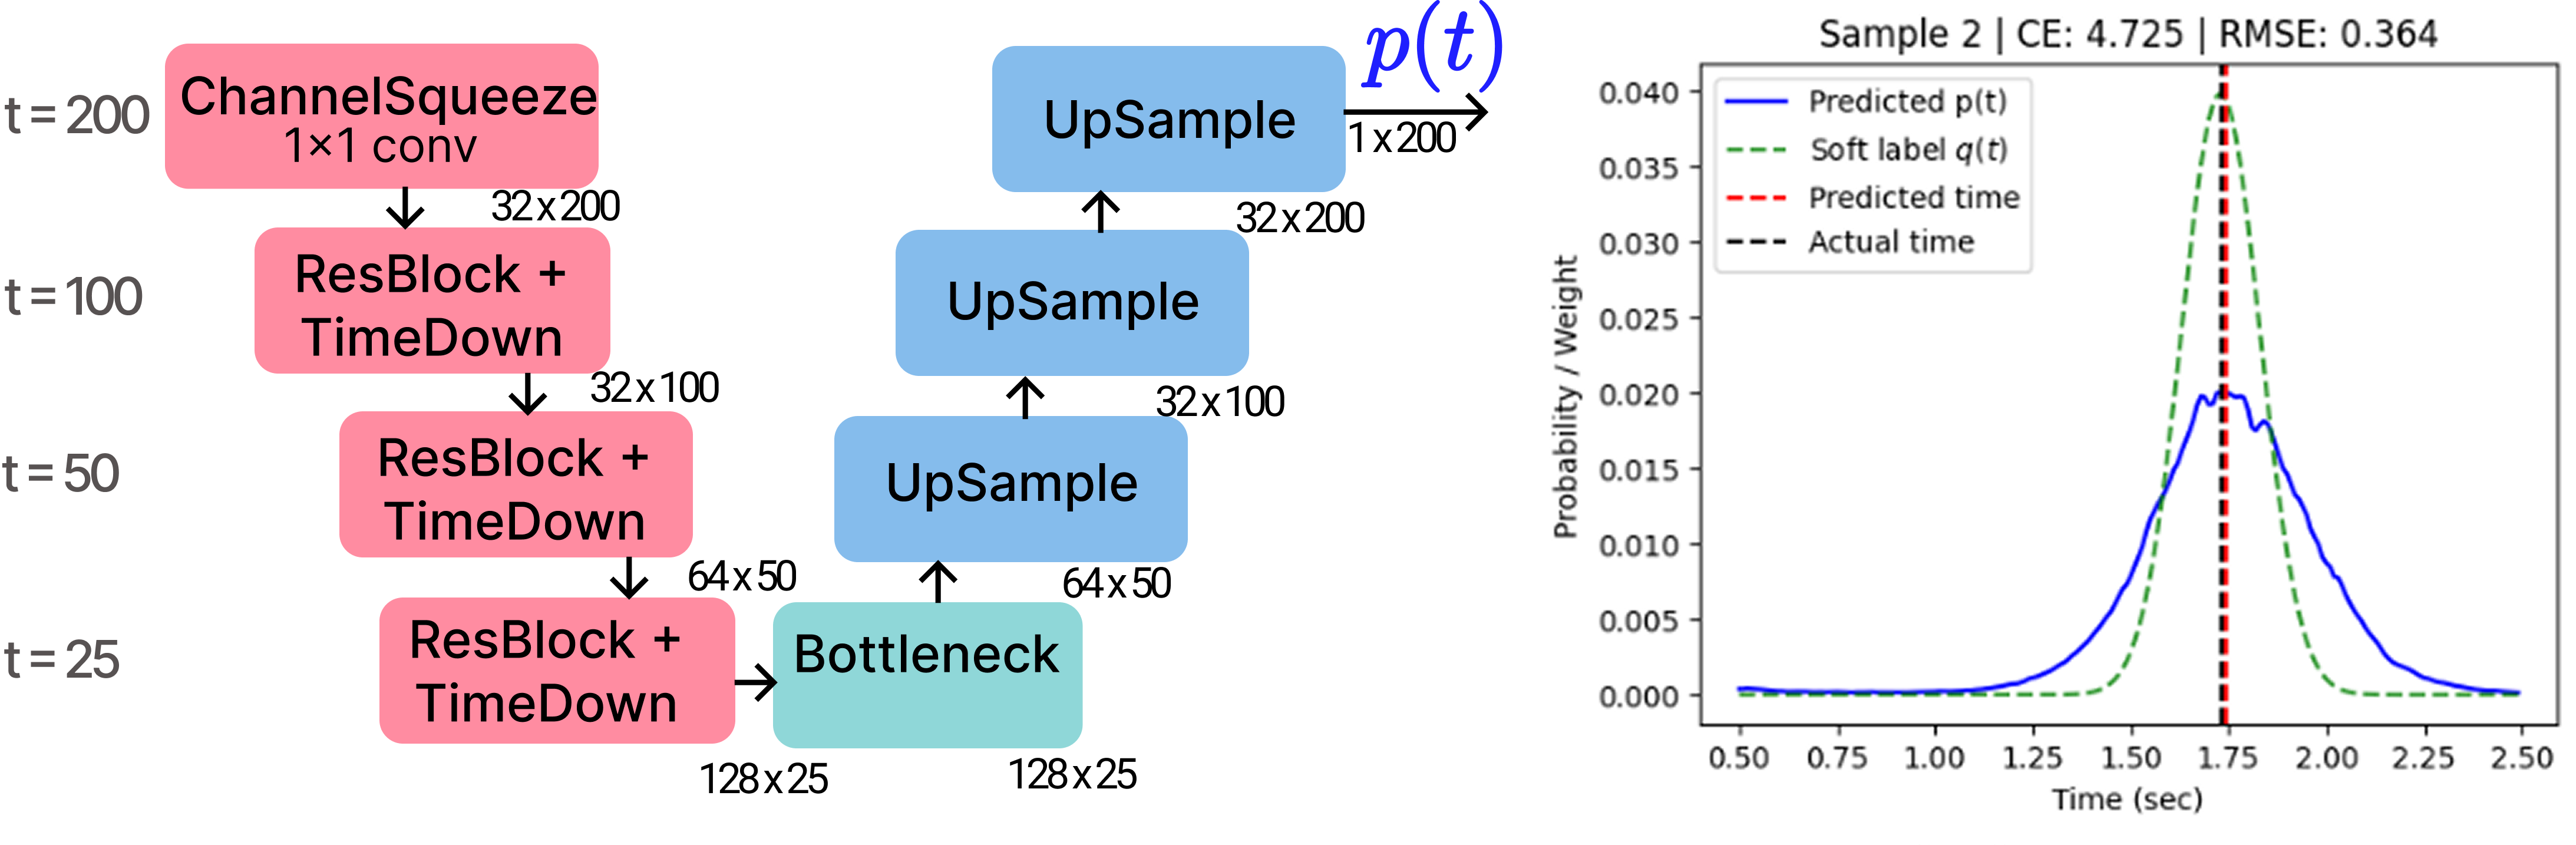
\includegraphics[width=0.9\linewidth]{img/ch1/Ch1_ets_unet_1.png}
    \caption{ETS-U-Net for RT segmentation. A lightweight 1-D U-Net maps an EEG trial window to per-time logits
    and an event-time distribution $p(t)$. The encoder applies a $1\times1$ channel-squeeze layer followed by residual
    blocks with temporal downsampling (\texttt{TimeDown}); a bottleneck aggregates context, and the decoder upsamples with
    skip connections to recover time-resolved outputs. The right panel shows an example prediction $p(t)$ and Gaussian soft
    target $q(t)$, together with the resulting predicted vs.\ observed response time.}
    \label{fig:ets_unet}
\end{figure}

\subsection{Soft-Target Event-Time Objectives}

Soft-target objectives instantiate the direct-supervision route: the observed RT is converted into a smooth target distribution over the represented time grid.

\paragraph{Soft target distribution.}
For each fixed 2~s input window, the observed RT \(y\) is converted into a
window-relative temporal target \(y_{\mathrm{rel}}=y-0.5\)~s on the represented
time grid.
A smooth segmentation label is constructed using a Gaussian kernel with bandwidth $\sigma$:
\begin{equation}
\label{eq:rt_soft_target}
\tilde q_t=\exp\left(-\frac{(g_t-y_{\mathrm{rel}})^2}{2\sigma^2}\right),\qquad
q_t=\frac{\tilde q_t}{\sum_{k=0}^{T-1}\tilde q_k},\qquad
\sum_{t=0}^{T-1} q_t=1.
\end{equation}
The Gaussian label avoids a degenerate single-bin target while keeping probability mass concentrated near the observed behavioral latency.

\paragraph{Model output and losses.}
Given logits $z_t$ for $t=0,\dots,T-1$, the predicted event-time distribution is obtained via temperature-scaled softmax,
\begin{equation}
\label{eq:rt_pred_dist}
p_t(\tau)=\frac{e^{z_t/\tau}}{\sum_{k=0}^{T-1} e^{z_k/\tau}}.
\end{equation}
The soft-label segmentation family is written as a weighted objective:
\begin{equation}
\label{eq:rt_loss}
\begin{aligned}
\mathcal{L}
&= \lambda_{\text{time}}\,\mathrm{RMSE}\big(\hat t_{\mathrm{rel}}(\tau), y_{\mathrm{rel}}\big)
 + \lambda_{\text{CE}}\,\mathrm{CE}\big(q, p(\tau)\big) \\
&\quad + \lambda_{W1}\,W_1\big(\mathrm{CDF}(q), \mathrm{CDF}(p(\tau))\big)
 + \lambda_{\text{KL}}\,D_{\mathrm{KL}}\big(q\|p(\tau)\big)
 + \lambda_{H}\,H\big(p(\tau)\big),
\end{aligned}
\end{equation}
where  
\begin{equation*}
\mathrm{CE}(q,p)=-\sum_{t=0}^{T-1} q_t \log p_t, \;
D_{\mathrm{KL}}(q\|p)=\sum_{t=0}^{T-1} q_t \log\frac{q_t}{p_t}, \;
H(p)=-\sum_{t=0}^{T-1} p_t \log p_t.
\end{equation*}
This expression defines an ablation family rather than a single prescribed loss. CE-only supervision sets the scalar time term to zero and asks the model to match a Gaussian soft event-time label. The soft-argmax RT-loss ablation removes distributional matching while keeping the same readout, and the Wasserstein-only ablation tests whether a CDF-based geometry loss is sufficient on its own. A CE+time hybrid is available by enabling both CE and soft-argmax time terms, but is not a separate row in the five-seed comparison. Entropy, KL, focal, and related terms serve as posterior-geometry controls when enabled.

\subsection{Likelihood-Based Event-Time Objectives}
\label{sec:event_nll}

As a probabilistic alternative to soft-target supervision, likelihood-based objectives model the observed scalar RT as a noisy realization of a latent response-relevant event time. Given the posterior over latent event bins, the marginal likelihood of the observed RT is
\begin{equation}
\label{eq:event_nll}
p(y\mid X)
= \sum_{t=0}^{T-1} p_t(X)\,
\mathcal{N}\!\left(y;\,t_0 + g_t,\,\sigma_y^2\right),
\qquad
\mathcal{L}_{\mathrm{EventNLL}} = -\log p(y\mid X).
\end{equation}
This objective keeps the same event-time interpretation but replaces the constructed target distribution $q_t$ with a marginal likelihood over latent response-relevant event times.

\paragraph{Observation-kernel and hazard extensions.}
The EventNLL formulation separates the latent event-time posterior $p_t(X)$ from the observation model $K(y\mid t)$. The default model uses a single Gaussian observation kernel, but we also evaluate a two-scale Gaussian mixture,
\begin{equation}
\label{eq:event_nll_mixture_kernel}
K(y\mid t)=(1-\alpha)\,\mathcal{N}(y;t_0+g_t,\sigma_{\mathrm{narrow}}^2)
+\alpha\,\mathcal{N}(y;t_0+g_t,\sigma_{\mathrm{wide}}^2),
\end{equation}
which keeps most probability mass in a narrow timing error while allowing a wider tail for occasional noisy RT observations. In the completed run, $\sigma_{\mathrm{narrow}}=0.10$~s, $\sigma_{\mathrm{wide}}=0.35$~s, and $\alpha=0.10$.

As a readout extension, we also evaluate a hazard/survival parameterization. Instead of using logits only as unconstrained softmax scores, each temporal logit defines a conditional event probability
\begin{equation}
\label{eq:hazard_readout}
h_t=\sigma(z_t/\tau),\qquad
p_t^{\mathrm{haz}} \propto h_t\prod_{k<t}(1-h_k),
\end{equation}
with the resulting event-bin probabilities normalized over the represented window. This keeps the same event-time likelihood in Eq.~\ref{eq:event_nll}, but changes the posterior parameterization from a categorical softmax to a discrete-time survival process. This extension tests whether the event-time formulation is tied to one softmax implementation.

\begin{table}[!htbp]
\centering
\caption{Event-time objective variants with a fixed ETS-U-Net backbone. Temperature is selected on R9--R10 for posterior-mean readout and then applied unchanged to the holdout split. Values are mean $\pm$ sample standard deviation over seeds 2025--2029.}
\label{tab:r11_segmentation_losses}
\footnotesize
\setlength{\tabcolsep}{2pt}
\renewcommand{\arraystretch}{1.15}
\begin{tabularx}{\linewidth}{@{} >{\RaggedRight\arraybackslash}p{0.18\linewidth} Y >{\centering\arraybackslash}p{0.17\linewidth} >{\centering\arraybackslash}p{0.17\linewidth} >{\centering\arraybackslash}p{0.17\linewidth} @{}}
\toprule
\textbf{Objective} & \textbf{Supervision signal} & \textbf{Valid nRMSE} & \textbf{Holdout nRMSE} & \textbf{Holdout \(\tau\)-nRMSE} \\
\midrule
\multicolumn{5}{@{}l}{\textit{Soft-target objectives}} \\
\addlinespace[0.15em]
CE & Gaussian soft event-time label & \mbox{0.8763 $\pm$ 0.0044} & \textbf{\mbox{0.8774 $\pm$ 0.0044}} & \mbox{0.8753 $\pm$ 0.0039} \\
\midrule
\multicolumn{5}{@{}l}{\textit{Likelihood-based objectives}} \\
\addlinespace[0.15em]
EventNLL & latent event time + Gaussian RT likelihood & \mbox{0.8769 $\pm$ 0.0030} & \mbox{0.8805 $\pm$ 0.0021} & \mbox{0.8772 $\pm$ 0.0018} \\
Mixture EventNLL & Two-component core-tail RT likelihood & \textbf{\mbox{0.8744 $\pm$ 0.0018}} & \mbox{0.8785 $\pm$ 0.0047} & \textbf{\mbox{0.8745 $\pm$ 0.0053}} \\
Hazard EventNLL & hazard posterior + Gaussian RT likelihood & \mbox{0.8755 $\pm$ 0.0027} & \mbox{0.8776 $\pm$ 0.0031} & \mbox{0.8778 $\pm$ 0.0041} \\
\midrule
\multicolumn{5}{@{}l}{\textit{Scalar-readout and distance controls}} \\
\addlinespace[0.15em]
Soft-argmax RT loss & posterior-mean RT error only; no distribution target & \mbox{0.8944 $\pm$ 0.0048} & \mbox{0.8943 $\pm$ 0.0025} & \mbox{0.8917 $\pm$ 0.0046} \\
Wasserstein & CDF match to Gaussian soft event-time label & \mbox{0.8997 $\pm$ 0.0035} & \mbox{0.8995 $\pm$ 0.0078} & \mbox{0.8896 $\pm$ 0.0033} \\
\bottomrule
\end{tabularx}
\end{table}
\FloatBarrier

\subsection{Formulation Comparison and Robustness}

The comparison in Table~\ref{tab:r11_segmentation_losses} evaluates the paper-facing ETS-U-Net objective variants under the fixed backbone and release-separated protocol. Here, holdout \(\tau\)-nRMSE denotes holdout nRMSE after applying the posterior-readout temperature \(\tau\) selected on R9--R10; holdout labels are used only for evaluation. The CE and likelihood-family objectives form the strongest scalar-readout group after readout-temperature tuning, with holdout \(\tau\)-nRMSE between 0.8745 and 0.8778. This improves over the strongest scalar regression baseline, ETR-CNN large (0.8928 $\pm$ 0.0042; Table~\ref{tab:r11_regression_baselines}), while the soft-argmax RT-loss and Wasserstein controls remain closer to the scalar-regression regime.

\paragraph{Objective ablations.}
The ablations separate expectation-style temporal readout from distributional supervision. The soft-argmax RT-loss control directly optimizes posterior-mean RT error but removes distribution matching; it remains close to the strongest scalar-regression baseline and trails the CE/EventNLL group by roughly 0.014--0.017 holdout \(\tau\)-nRMSE. CE and the likelihood-family variants form a tight top group: mixture EventNLL has the best mean temperature-tuned scalar readout, but CE, Gaussian EventNLL, mixture EventNLL, and hazard EventNLL are close relative to seed variability. The hazard result shows that the likelihood-family conclusion is not tied to a categorical softmax posterior, while the Wasserstein control shows that an alternative distributional distance alone does not match the CE/EventNLL scalar readouts. Thus, the central gain is best attributed to distributional event-time supervision rather than to the U-Net backbone or soft-argmax readout alone.

\paragraph{Practical effect size.}
To quantify the practical size of the main accuracy gain, we compared the strongest scalar baseline, ETR-CNN large, with the strongest event-time objectives using matched seeds and subject-level bootstrap intervals on the holdout split. Mixture EventNLL reduced \(\tau\)-nRMSE from \(0.8928 \pm 0.0042\) to \(0.8745 \pm 0.0053\), an absolute reduction of \(0.0184\), or about \(2.1\%\) relative improvement. On the RT scale, this corresponds to a \(6.24\)~ms reduction in RMSE and an \(8.94\)~ms reduction in MAE, with subject-bootstrap 95\% confidence intervals of \([4.50, 7.97]\)~ms and \([7.43, 10.49]\)~ms, respectively. The gain was positive for all five matched-seed comparisons. Thus, the scalar accuracy gain is moderate in absolute milliseconds but consistent across seeds and subjects. The event-time formulation also provides posterior diagnostics and shifted-crop analyses that are not available from scalar regression alone.

\begin{figure}[!t]
    \centering
    
\includegraphics[width=0.88\linewidth]{img/ch1/trial_sorted_posterior_raster.png}
    \caption{Trial-sorted event-time posterior maps on the holdout split for matched segmentation losses. Rows are quantile bins of representable holdout trials sorted by observed RT; the x-axis is time from stimulus onset; color shows log-transformed posterior density averaged within each bin. The overlaid curve marks the mean observed RT in each bin.}
    \label{fig:posterior_raster_main}
\end{figure}

\section{Posterior Readout and Diagnostics}
\label{sec:posterior_diagnostics}

\subsection{Scalar Readout and Temperature Tuning}

Event-time models output a posterior over response-relevant time bins, whereas the benchmark evaluates scalar RT. We therefore use the posterior expectation as the scalar readout: the predicted relative time is the probability-weighted average of the temporal grid, and the absolute RT is obtained by adding the fixed window start time,
\begin{equation}
\label{eq:rt_soft_argmax}
\hat t_{\mathrm{rel}}(\tau)=\sum_{t=0}^{T-1} p_t(\tau)\, g_t,
\qquad
\hat t_{\mathrm{abs}}(\tau)=t_0+\hat t_{\mathrm{rel}}(\tau),
\end{equation}
where $g_t=t\,\Delta t$ denotes the discrete time grid. This readout is aligned with squared-error evaluation and keeps event-time models comparable to scalar regression baselines under nRMSE.

Because different objectives can produce posteriors with different sharpness, we select a readout temperature on the R9--R10 development split to minimize nRMSE of the posterior-mean prediction, and apply the selected temperature unchanged to the holdout set:
\begin{equation}
\label{eq:rt_tau_tuning}
\tau_m^\star = \arg\min_{\tau\in\mathcal{T}_{\text{cal}}}
\ \mathrm{nRMSE}_{\text{val}}\big(\hat t_{\mathrm{abs}}^{(m)}(\tau)\big).
\end{equation}
The resulting scalar value is reported as holdout \(\tau\)-nRMSE in Table~\ref{tab:r11_segmentation_losses}. This temperature step is a scalar-readout protocol, not full probabilistic calibration; likelihood, coverage, and posterior concentration are evaluated separately below.

\subsection{Posterior Geometry Diagnostics}

Once the scalar readout has been fixed, the event-time posterior makes temporally resolved evaluation possible rather than limiting assessment to point prediction. Scalar nRMSE asks whether the posterior mean predicts RT accurately, but similar nRMSE values can hide very different temporal evidence. Posterior geometry asks where the model places probability mass, whether that mass is localized near the observed behavioral latency, whether the posterior peak agrees with the posterior mean, and whether nominal posterior intervals have meaningful empirical coverage.

We first inspect the trial-sorted posterior maps in Figure~\ref{fig:posterior_raster_main} before reducing the posterior to summary metrics. These maps show the full distribution over response-relevant event time for holdout trials ordered by observed RT, rather than only the posterior mean. CE and Wasserstein place broad probability mass across the response window, whereas the EventNLL-family objectives produce sharper probability bands that more closely track the observed RT curve. This qualitative pattern motivates the quantitative posterior-geometry summaries in Figure~\ref{fig:posterior_geometry_main} and Table~\ref{tab:posterior_geometry_metrics}.

Table~\ref{tab:posterior_geometry_metrics} reduces the posterior maps to four complementary diagnostic families. First, nRMSE asks whether the posterior mean remains a good scalar RT predictor. Second, fixed-kernel EventNLL evaluates the full posterior as a distribution by scoring the observed RT under a common Gaussian observation kernel. Third, Width80 and Mass $\pm$150 ms describe localization: whether probability mass is diffuse or concentrated near the behavioral latency. Finally, Coverage80 and Coverage MAE assess interval reliability, asking whether nominal posterior intervals contain the observed RT at the expected rates. These metrics are not intended to produce a single ranking; they expose trade-offs among scalar accuracy, posterior sharpness, target alignment, and calibration.

Figure~\ref{fig:posterior_geometry_main} visualizes this trade-off space before the exact values are tabulated. The key pattern is not a single dominant objective: scalar nRMSE remains close for the leading losses, while posterior concentration, target-aligned mass, and interval coverage separate them into different regimes.

\begin{figure}[!t]
    \centering
    
\includegraphics[width=\linewidth]{img/ch1/posterior_geometry_main.png}
    \caption{Posterior geometry differs across event-time losses even when scalar nRMSE is similar. Panel A reports holdout scalar readout after selecting the softmax temperature on R9--R10 to minimize nRMSE. Panel B aligns predicted posteriors to the observed RT. Panels C--E summarize posterior width, near-target mass, and mode-mean disagreement. Panel F compares empirical coverage of central posterior intervals; the diagonal is ideal interval coverage.}
    \label{fig:posterior_geometry_main}
\end{figure}

These diagnostics show that losses with similar scalar error can induce different posterior semantics. CE and mixture EventNLL provide the strongest scalar readouts. EventNLL-family objectives are sharper and more target-concentrated, but they under-cover nominal intervals. The soft-argmax RT-loss control has the lowest Coverage MAE because its posterior is broad, but it is weaker as a scalar predictor and lacks distributional event-time supervision. Wasserstein is closest to nominal 80\% coverage, but it has weaker scalar accuracy and lower near-target mass. Thus, posterior geometry reveals trade-offs among scalar accuracy, target concentration, distributional scoring, and interval behavior that scalar nRMSE alone would hide.

Consequently, the preferred event-time objective depends on the downstream goal rather than on a single universal ranking. If the goal is scalar RT prediction, CE and mixture EventNLL are the strongest choices in this study. If the goal is a sharper posterior concentrated near the observed behavioral latency, the EventNLL-family objectives are more appropriate, although their nominal intervals under-cover. If interval reliability is the priority, broader objectives such as Wasserstein or the soft-argmax RT-loss control give better coverage behavior, but with weaker scalar accuracy or weaker distributional event-time supervision. The shifted-crop analysis below further shows that crop-relative movement is partly separable from scalar error, posterior concentration, and interval coverage.

\begin{table}[!htbp]
\centering
\caption{Quantitative posterior geometry on the holdout split for matched event-time segmentation losses. Values are mean $\pm$ standard deviation across seeds after R9--R10 readout-temperature selection; arrows indicate the preferred direction, Coverage80 is best when close to 0.80, and bold marks the best point estimate per metric.}
\label{tab:posterior_geometry_metrics}
\scriptsize
\setlength{\tabcolsep}{3pt}
\renewcommand{\arraystretch}{1.12}
\resizebox{\linewidth}{!}{%
\begin{tabular}{@{} l c c c c c c @{}}
\toprule
\textbf{Objective} & \textbf{nRMSE $\downarrow$} & \textbf{Fixed NLL $\downarrow$} & \textbf{Width80 ms $\downarrow$} & \textbf{Mass $\pm$150 ms $\uparrow$} & \textbf{Coverage80} & \textbf{Coverage MAE $\downarrow$} \\
\midrule
CE & 0.875 $\pm$ 0.004 & 0.08 $\pm$ 0.01 & 766 $\pm$ 36 & 0.334 $\pm$ 0.008 & 0.883 $\pm$ 0.013 & 0.101 $\pm$ 0.014 \\
EventNLL & 0.877 $\pm$ 0.002 & -0.06 $\pm$ 0.01 & 502 $\pm$ 15 & 0.490 $\pm$ 0.008 & 0.500 $\pm$ 0.025 & 0.273 $\pm$ 0.021 \\
Mixture EventNLL & \textbf{0.874 $\pm$ 0.005} & \textbf{-0.08 $\pm$ 0.01} & 528 $\pm$ 22 & 0.471 $\pm$ 0.008 & 0.573 $\pm$ 0.020 & 0.207 $\pm$ 0.017 \\
Hazard EventNLL & 0.878 $\pm$ 0.004 & -0.06 $\pm$ 0.01 & \textbf{445 $\pm$ 14} & \textbf{0.502 $\pm$ 0.005} & 0.468 $\pm$ 0.007 & 0.302 $\pm$ 0.006 \\
Soft-argmax RT loss & 0.892 $\pm$ 0.005 & 0.11 $\pm$ 0.03 & 844 $\pm$ 96 & 0.357 $\pm$ 0.015 & 0.843 $\pm$ 0.029 & \textbf{0.040 $\pm$ 0.024} \\
Wasserstein & 0.890 $\pm$ 0.003 & 0.20 $\pm$ 0.04 & 632 $\pm$ 101 & 0.334 $\pm$ 0.028 & \textbf{0.774 $\pm$ 0.061} & 0.059 $\pm$ 0.021 \\
\bottomrule
\end{tabular}%
}
\end{table}

\subsection{Shifted-Crop Shortcut-vs-Localization Diagnostic}

Posterior geometry characterizes how probability mass is arranged inside the standard stimulus-locked window. It does not, by itself, test whether the prediction behaves like a crop-relative timing localizer when the temporal frame of reference changes. A fixed-window model can still exploit shortcuts: trial difficulty, subject-level response tendency, or stimulus-locked timing structure may support scalar RT prediction without requiring within-window response-timing localization.

We therefore use shifted-crop inference as a shortcut-vs-localization diagnostic on the holdout split. For each trial, we take the same 5~s EEG cache and evaluate the trained model on 2~s crops starting at $s\in\{0.2,0.3,\dots,0.8\}$~s after stimulus onset. The standard inference window corresponds to $s=0.5$~s. For a crop starting at $s$, the crop-relative target is $\mathrm{RT}-s$. A model that localizes response-relevant timing within the crop should adjust its crop-relative prediction when the crop start changes; a shortcut model tied to stimulus-locked scalar timing should be less sensitive to this perturbation.

Table~\ref{tab:shift_jitter_summary} summarizes this diagnostic together with a matched shift-jitter intervention. Shifted relative nRMSE measures crop-relative prediction accuracy across shifted crops. Sensitivity quantifies the fraction of the imposed crop shift reflected in the prediction, with 1 indicating ideal crop-relative localization and 0 indicating crop-invariant behavior. Direction is the fraction of shifted examples whose prediction moves in the expected localizer direction. Accuracy metrics are computed over crop examples in which the behavioral response remains observable within the evaluated 2~s window, whereas sensitivity and direction use the common trial subset for which the response remains inside every evaluated crop.

\begin{table}[!hbp]
\centering
\caption{Shifted-crop diagnostic and shift-jitter intervention on the 5~s holdout dataset. Values are seed means; full mean $\pm$ standard deviation values are reported in Appendix Table~\ref{tab:shift_jitter_summary_full}. Arrows indicate the preferred direction.}
\label{tab:shift_jitter_summary}
\footnotesize
\setlength{\tabcolsep}{3.5pt}
\renewcommand{\arraystretch}{1.12}
\begin{tabular}{@{} l c c c c c c c c @{}}
\toprule
\textbf{Objective} & \multicolumn{2}{c}{\textbf{Holdout \(\tau\)-nRMSE} $\downarrow$} & \multicolumn{2}{c}{\textbf{Shifted rel. nRMSE} $\downarrow$} & \multicolumn{2}{c}{\textbf{Sensitivity} $\uparrow$} & \multicolumn{2}{c}{\textbf{Direction} $\uparrow$} \\
\cmidrule(lr){2-3}\cmidrule(lr){4-5}\cmidrule(lr){6-7}\cmidrule(l){8-9}
 & \textbf{Fixed} & \textbf{Jitter} & \textbf{Fixed} & \textbf{Jitter} & \textbf{Fixed} & \textbf{Jitter} & \textbf{Fixed} & \textbf{Jitter} \\
\midrule
CE & 0.8753 & 0.8749 & 0.8679 & \textbf{0.8569} & 0.5810 & 0.5831 & 0.7780 & 0.7924 \\
Mixture EventNLL & \textbf{0.8745} & \textbf{0.8734} & \textbf{0.8663} & 0.8576 & 0.6021 & 0.6249 & 0.7730 & 0.7925 \\
EventNLL & 0.8772 & 0.8771 & 0.8685 & 0.8593 & 0.5842 & 0.6174 & 0.7739 & 0.7937 \\
Hazard EventNLL & 0.8778 & 0.8806 & 0.8692 & 0.8609 & 0.5618 & 0.5891 & 0.7694 & 0.7925 \\
Soft-argmax RT loss & 0.8917 & 0.8836 & 0.8857 & 0.8613 & 0.5381 & 0.5775 & 0.7592 & 0.7951 \\
Wasserstein & 0.8896 & 0.8922 & 0.8932 & 0.8774 & \textbf{0.6684} & \textbf{0.6852} & \textbf{0.7830} & \textbf{0.8026} \\
\bottomrule
\end{tabular}
\end{table}

We then trained matched shift-jitter variants in which the 2~s training window was sampled from the same crop-start range and the target was expressed relative to the sampled window. The intervention does not produce a broad ordinary-holdout gain under the canonical support: CE, mixture EventNLL, and Gaussian EventNLL remain essentially unchanged in holdout \(\tau\)-nRMSE. Its main effect is instead on shifted-crop behavior. Shifted relative nRMSE improves for every objective, and direction consistently increases, indicating that predictions more often move in the expected localizer direction. Sensitivity also improves modestly, but remains well below the ideal value of 1.

Across objectives, Wasserstein is the most localizer-like by sensitivity and direction, but this comes with weaker scalar and shifted-crop accuracy. This reinforces the broader trade-off exposed by the posterior analyses: objectives that encourage stronger crop-relative movement need not be the best point predictors. Overall, shift-jitter reduces fixed-window shortcut behavior without turning these models into fully shift-equivariant response-timing localizers.

\FloatBarrier

\section{Discussion}

\subsection{Event-Time Supervision and Objective Geometry}

The results support treating trial-wise RT prediction as event-time posterior modeling rather than as ordinary scalar regression. The label is a behavioral latency within a post-stimulus interval, and models benefit when that temporal structure is explicit in the output space and in the loss. CE and the EventNLL-family objectives form the strongest scalar-readout group, whereas the soft-argmax RT-loss control is weaker despite using the same posterior-mean readout. This supports the interpretation that the gain comes from distributional event-time supervision, not merely from replacing a scalar head with a differentiable expectation.

The objective comparison also shows that event-time losses do not all impose the same computational semantics. CE-style soft targets provide strong scalar readouts and broad posterior support. EventNLL reaches a similar scalar-error regime through a latent-variable likelihood, marginalizing an unobserved response-relevant event time under an observation model for RT. Wasserstein behaves differently: it is more localizer-like by shifted-crop sensitivity and direction, but weaker as a point predictor. Thus, the choice of objective controls a trade-off among scalar accuracy, posterior concentration, interval behavior, and crop-relative movement.

The wrapped external baselines show that standardized EEG architectures can train under the same fixed-normalization protocol, but they do not close the gap to compact task-specific models or event-time segmentation. Foundation-style architectures are evaluated here as architectures trained from scratch, not as pretrained models. The comparison is therefore not a test of pretraining; it shows that, under this benchmark protocol, formulation and objective design are strong levers even with lightweight supervised models.

\subsection{Posterior Diagnostics and Shifted-Crop Behavior}

The event-time posterior contains more information than its expectation. Posterior width, target-aligned mass, mode-mean disagreement, fixed-kernel EventNLL, and interval coverage expose temporal output behavior that scalar nRMSE discards. This is important because similar point errors can correspond to different posterior semantics: broad conservative distributions, sharper target-concentrated distributions, or better interval coverage with weaker scalar prediction.

Temperature tuning should therefore be interpreted narrowly. In this study, temperature is a scalar-readout protocol for comparing posterior-mean predictions under nRMSE. It is not the main methodological claim and does not replace distributional diagnostics. Likelihood, coverage, posterior concentration, and shifted-crop behavior are evaluated separately because they answer different questions about the learned event-time posterior. Objective choice remains a downstream trade-off among point prediction, target concentration, interval reliability, and crop-relative movement.

The shifted-crop diagnostic extends this posterior analysis from shape to behavior under temporal perturbation. If fixed-window training permits stimulus-locked shortcuts, then crop shifts should reveal whether predictions move in a crop-relative, localizer-like direction. Shift-jitter training targets this failure mode directly by varying the crop start during training and expressing the target relative to the sampled crop. Its main effect is not a broad improvement in ordinary fixed-window holdout nRMSE, but improved shifted-crop robustness and more frequent movement in the expected localizer direction. Sensitivity remains well below the ideal value of 1, so shift-jitter reduces fixed-window shortcut behavior without solving fully shift-equivariant response-timing localization.

\subsection{Scope and Limitations}

The main limitation is that all claims are tied to the HBN-EEG contrast change detection task and the release-separated protocol used here. The final holdout release is stronger than reused validation performance, but it is still drawn from the same broader dataset family and preprocessing pipeline. Broader claims about EEG event-time modeling require replication across tasks, acquisition settings, montages, and latency targets.

The shifted-crop results should also be interpreted as partial response-timing localization evidence rather than solved neural event detection. Even after shift-jitter training, sensitivity remains far from the ideal crop-relative localizer. Stronger localization claims will require training objectives, architectures, or augmentations designed explicitly for temporal equivariance. The five-seed robustness checks support the main scalar-versus-event-time comparison, but they cover selected core recipes rather than every kernel, hazard, calibration, and architecture variant. The foundation-style comparisons also do not use pretrained weights or montage-specialized setup changes; they are controlled architecture baselines rather than a full evaluation of EEG foundation models.

Taken together, these results support event-time posterior modeling as a computational bridge between behavioral latency prediction and event-centered EEG analysis. The framework improves scalar RT decoding, exposes posterior structure hidden by nRMSE, and enables shortcut-vs-localization diagnostics under temporal perturbation. At the same time, the shifted-crop results make the remaining gap explicit: current fixed-window models become more localizer-like, especially under shift-jitter training, but they do not yet implement full crop-relative response-timing localization.

\section{Conclusion}

We reformulated EEG-based reaction-time prediction as event-time posterior modeling and evaluated it under a release-separated HBN-EEG protocol. The results indicate that supervising an event-time posterior improves RT prediction beyond scalar regression and beyond a temporal-readout head alone. Loss ablations and five-seed robustness checks show that distributional event-time supervision matters, EventNLL provides a principled latent-variable likelihood alternative, and posterior-geometry plus shifted-crop analyses reveal output behavior that scalar nRMSE alone cannot capture.

\appendix

\section{Additional Posterior Geometry Examples}

Table~\ref{tab:posterior_geometry_metrics} reports the quantitative posterior metrics behind Figure~\ref{fig:posterior_geometry_main}, and Figure~\ref{fig:posterior_raster_main} shows the corresponding trial-sorted posterior maps in the main text. Figure~\ref{fig:appendix_temperature_sensitivity} shows the development-split temperature curves used to choose post-hoc readout temperatures.

\begin{figure}[!t]
    \centering
    
\includegraphics[width=0.9\linewidth]{img/ch1/temperature_sensitivity.png}
    \caption{Temperature sensitivity on the R9-R10 development split. Vertical lines mark selected temperatures. The curves show that different losses induce different confidence scales, motivating a fixed readout-temperature selection protocol before comparing posterior-mean scalar readouts or posterior diagnostics.}
    \label{fig:appendix_temperature_sensitivity}
\end{figure}

\begin{table}[!htbp]
\centering
\caption{Full shifted-crop diagnostic and shift-jitter intervention summary with seed variability. Values are mean $\pm$ standard deviation across seeds; the corresponding main-text table reports means only for readability.}
\label{tab:shift_jitter_summary_full}
\scriptsize
\setlength{\tabcolsep}{2.2pt}
\renewcommand{\arraystretch}{1.12}
\resizebox{\linewidth}{!}{%
\begin{tabular}{@{} l c c c c c c c c @{}}
\toprule
\textbf{Objective} & \multicolumn{2}{c}{\textbf{Holdout \(\tau\)-nRMSE} $\downarrow$} & \multicolumn{2}{c}{\textbf{Shifted rel. nRMSE} $\downarrow$} & \multicolumn{2}{c}{\textbf{Sensitivity} $\uparrow$} & \multicolumn{2}{c}{\textbf{Direction} $\uparrow$} \\
\cmidrule(lr){2-3}\cmidrule(lr){4-5}\cmidrule(lr){6-7}\cmidrule(l){8-9}
 & \textbf{Fixed} & \textbf{Jitter} & \textbf{Fixed} & \textbf{Jitter} & \textbf{Fixed} & \textbf{Jitter} & \textbf{Fixed} & \textbf{Jitter} \\
\midrule
CE & 0.8753 $\pm$ 0.0039 & 0.8749 $\pm$ 0.0060 & 0.8679 $\pm$ 0.0024 & 0.8569 $\pm$ 0.0060 & 0.5810 $\pm$ 0.0351 & 0.5831 $\pm$ 0.0406 & 0.7780 $\pm$ 0.0041 & 0.7924 $\pm$ 0.0056 \\
Mixture EventNLL & 0.8745 $\pm$ 0.0053 & 0.8734 $\pm$ 0.0033 & 0.8663 $\pm$ 0.0037 & 0.8576 $\pm$ 0.0041 & 0.6021 $\pm$ 0.0484 & 0.6249 $\pm$ 0.0313 & 0.7730 $\pm$ 0.0062 & 0.7925 $\pm$ 0.0076 \\
EventNLL & 0.8772 $\pm$ 0.0018 & 0.8771 $\pm$ 0.0040 & 0.8685 $\pm$ 0.0023 & 0.8593 $\pm$ 0.0028 & 0.5842 $\pm$ 0.0287 & 0.6174 $\pm$ 0.0222 & 0.7739 $\pm$ 0.0059 & 0.7937 $\pm$ 0.0068 \\
Hazard EventNLL & 0.8778 $\pm$ 0.0041 & 0.8806 $\pm$ 0.0034 & 0.8692 $\pm$ 0.0028 & 0.8609 $\pm$ 0.0045 & 0.5618 $\pm$ 0.0376 & 0.5891 $\pm$ 0.0259 & 0.7694 $\pm$ 0.0090 & 0.7925 $\pm$ 0.0074 \\
Soft-argmax RT loss & 0.8917 $\pm$ 0.0046 & 0.8836 $\pm$ 0.0035 & 0.8857 $\pm$ 0.0069 & 0.8613 $\pm$ 0.0032 & 0.5381 $\pm$ 0.0586 & 0.5775 $\pm$ 0.0362 & 0.7592 $\pm$ 0.0183 & 0.7951 $\pm$ 0.0052 \\
Wasserstein & 0.8896 $\pm$ 0.0033 & 0.8922 $\pm$ 0.0066 & 0.8932 $\pm$ 0.0033 & 0.8774 $\pm$ 0.0099 & 0.6684 $\pm$ 0.0711 & 0.6852 $\pm$ 0.0416 & 0.7830 $\pm$ 0.0197 & 0.8026 $\pm$ 0.0118 \\
\bottomrule
\end{tabular}%
}
\end{table}

\section{Reproducibility Details}
\label{app:reproducibility_details}

All paper-facing experiments are specified by YAML configuration files under \texttt{benchmarks/configs/} and write run summaries, prediction files, selected temperatures, and model summaries under \texttt{benchmarks/experiments/}. Table~\ref{tab:reproducibility_details} summarizes the shared settings needed to reproduce the controlled comparisons: data splits, input representation, optimization, augmentation, model selection, readout-temperature tuning, and the main architecture hyperparameters. Settings not listed in the table are objective-specific loss choices described in the main text.

\begin{table}[!htbp]
\centering
\caption{Reproducibility summary for the main controlled comparisons.}
\label{tab:reproducibility_details}
\scriptsize
\setlength{\tabcolsep}{4pt}
\renewcommand{\arraystretch}{1.12}
\begin{tabularx}{\linewidth}{@{} p{0.20\linewidth} p{0.25\linewidth} X @{}}
\toprule
\textbf{Group} & \textbf{Setting} & \textbf{Value} \\
\midrule
\multicolumn{3}{@{}l}{\textit{Data and splits}} \\
\addlinespace[0.15em]
Input window & EEG segment & 0.5--2.5~s after stimulus onset; 2~s, 200 samples, 100~Hz, 128 channels. \\
Target support & Main analyzed set & \(0.5 \leq \mathrm{RT} \leq 2.5\)~s. \\
Splits & Release-separated protocol & R1--R8 train, R9--R10 development, R11 final holdout. \\
Seeds & Repeated runs & 2025--2029. \\
\midrule
\multicolumn{3}{@{}l}{\textit{Optimization and selection}} \\
\addlinespace[0.15em]
Optimizer & Neural models & Adam, learning rate \(10^{-3}\), weight decay 0. \\
Training loop & Epochs and batch size & Maximum 100 epochs; train batch size 128. \\
Evaluation loader & Batch size & Development and holdout batch size 256. \\
Checkpoint selection & Model selection & Best development nRMSE; early stopping patience 20. \\
Holdout use & Final evaluation & R11 is evaluated after checkpoint and readout choices are fixed. \\
Confidence intervals & Holdout summaries & Subject bootstrap over R11 subjects; 1000 samples for per-run intervals and 5000 samples for the scalar effect-size analysis. \\
\midrule
\multicolumn{3}{@{}l}{\textit{Training augmentations}} \\
\addlinespace[0.15em]
Channel dropout & Shared training augmentation & Applied with probability 0.25; dropped-channel ratio sampled uniformly from 0 to 0.3. \\
Temporal cutout & Shared training augmentation & Applied with probability 0.25; contiguous zeroed segment length 10--50 samples. \\
Gaussian noise & Shared training augmentation & Applied with probability 0.30; noise standard deviation \(0.01 + 0.01|\mathcal{N}(0,1)|\). \\
Time scaling & Fixed-window main runs & Disabled (\(p=0\)). \\
Mixup & All paper-facing runs & Disabled (\(p=0\)). \\
Shift-jitter & Intervention runs only & Training crop start sampled from 0.2--0.8~s, crop length 2~s, target expressed relative to crop start. \\
\midrule
\multicolumn{3}{@{}l}{\textit{Event-time readout}} \\
\addlinespace[0.15em]
Event grid & Temporal support & 200 bins over 2~s; 10~ms per bin. \\
Soft target & Gaussian event-time label & \(\sigma=0.15\)~s. \\
Posterior readout & Scalar prediction & Posterior mean / soft-argmax. \\
Base temperature & Training/evaluation default & \(\tau=0.65\) before post-hoc readout-temperature selection. \\
Temperature selection & Readout tuning & Grid search on R9--R10 minimizing posterior-mean nRMSE; selected \(\tau\) applied unchanged to R11. \\
Temperature grid & Objective-specific grid & \(0.4\)--\(1.8\) with step 0.05 for CE/EventNLL/soft-argmax RT-loss objectives; \(0.2\)--\(3.5\) with step 0.05 for Wasserstein. \\
\midrule
\multicolumn{3}{@{}l}{\textit{Core architectures}} \\
\addlinespace[0.15em]
ETS-U-Net & Event-time backbone & \(c_0=96\), widen 2, depth per stage 5, kernel size 15, dropout 0.2, one output channel; 3.10M parameters. \\
ETR-CNN large & Strongest scalar baseline & \(c_0=96\), widen 3, kernel size 15, dropout 0.2, high-resolution depth 12, low-resolution depth 10, three low-resolution stacks, two downsampling stages; 12.87M parameters. \\
ETR-CNN & Scalar temporal-readout baseline & Same family as ETR-CNN large with \(c_0=64\); 5.91M parameters. \\
MSP-CNN & Segment-pooling scalar baseline & \(c_0=48\), widen 2, depth per stage 3, kernel size 15, dropout 0.05; 3.01M parameters. \\
\bottomrule
\end{tabularx}
\end{table}

Wrapped external EEG architectures are instantiated from the YAML-specified Braindecode constructors and trained from scratch under the same data split, target support, optimizer, augmentation, checkpoint-selection, and holdout-evaluation protocol. Seed-level summaries, selected readout temperatures, prediction files, and paper-facing aggregate tables are stored under \texttt{benchmarks/experiments/}.


\FloatBarrier
\clearpage
\bibliography{../references}






% \bibliographystyle{APA}
% \begin{thebibliography}{100}
% \providecommand{\natexlab}[1]{#1}
% \expandafter\ifx\csname urlstyle\endcsname\relax
%   \providecommand{\doi}[1]{doi:\discretionary{}{}{}#1}\else
%   \providecommand{\doi}{doi:\discretionary{}{}{}\begingroup
%   \urlstyle{rm}\Url}\fi

% \bibitem[{LastName(2009)}]{Ref2009}
% LastName, A. (2009).
% \newblock Title for the first reference.
% \newblock \emph{Journal of the first reference}, \emph{3}, 18 -- 88.


% \bibitem[{Authors et~al.(2008)Author1, Author2, \&
%   Author3}]{Ref2008}
% Author1, A., Author2, A., \& Author3, A. (2008).
% \newblock Title for the second reference.
% \newblock \emph{Journal for the second reference}, \emph{5}, 188 -- 200.

% \end{thebibliography}
\end{document}
